
\section{Sicherungen}
\label{section:sicherungen}
\begin{frame}%STARTCONTENT

\begin{columns}
    \begin{column}{0.48\textwidth}
    \begin{itemize}
  \item Im Netzgerät und/oder in der Verbindungsleitung zum Transceiver gibt es sogenannte Feinsicherungen
  \item Diese unterbrechen im Fehlerfall (Kurzschluss oder Überlastung) den Stromfluss
  \end{itemize}

    \end{column}
   \begin{column}{0.48\textwidth}
       
\begin{figure}
    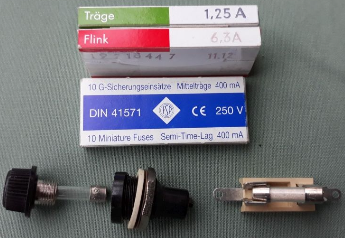
\includegraphics[width=0.85\textwidth]{foto/88}
    \caption{\scriptsize Feinsicherungen}
    \label{n_feinsicherungen}
\end{figure}

   \end{column}
\end{columns}

\end{frame}

\begin{frame}\begin{itemize}
  \item Nachdem eine Feinsicherung ausgelöst hat und man die Ursache behoben hat, muss man sie austauschen.
  \item Defekte Sicherungen dürfen \emph{nur durch gleichartige ersetzt werden}!
  \item Dabei ist sowohl auf \emph{Stromstärke} als auch die \emph{Auslösecharakteristik} zu achten, die angibt, wie schnell eine Sicherung auslöst (flink, mittelträge, träge).
  \end{itemize}
\end{frame}

\begin{frame}\begin{table}
\begin{DARCtabular}{ccc}
     Auslösecharakteristik  & Kennzeichen  & Abschaltzeit bei zehnfachem Nennstrom   \\
     flink  & F  & max. 30 ms  \\
     mittelträge  & MT  & max. 90 ms   \\
     träge  & T  & max. 300 ms   \\
\end{DARCtabular}
\caption{Kenngrößen von Feinsicherungen}
\label{n_feinsicherung}
\end{table}
\end{frame}

\begin{frame}
\only<1>{
\begin{QQuestion}{EK204}{Sie haben in ihren Kurzwellensender soeben einen Kurzschluss im Netzteil erfolgreich repariert. Durch den Fehler wurde auch die Feinsicherung für die Stromversorgung mit der Aufschrift \qty{20}{\A} \glqq Flink\grqq{} zerstört. Beim Austausch dieser Sicherung~...}{darf der Stromwert auch größer als \qty{20}{\A} sein, es muß jedoch eine Sicherung mit Auslösecharakteristik \glqq Flink\grqq{} eingesetzt werden.}
{darf bei gleichem Stromwert auch eine Sicherung mit Auslösecharakteristik \glqq Mittelträge\grqq{} oder \glqq Träge\grqq{} eingesetzt werden.}
{sollte eine Sicherung gleichen Stromwertes und gleicher Auslösecharakteristik eingesetzt werden.}
{kann ersatzweise auch eine Drahtbrücke aus dünnem Kupferdraht eingesetzt werden.}
\end{QQuestion}

}
\only<2>{
\begin{QQuestion}{EK204}{Sie haben in ihren Kurzwellensender soeben einen Kurzschluss im Netzteil erfolgreich repariert. Durch den Fehler wurde auch die Feinsicherung für die Stromversorgung mit der Aufschrift \qty{20}{\A} \glqq Flink\grqq{} zerstört. Beim Austausch dieser Sicherung~...}{darf der Stromwert auch größer als \qty{20}{\A} sein, es muß jedoch eine Sicherung mit Auslösecharakteristik \glqq Flink\grqq{} eingesetzt werden.}
{darf bei gleichem Stromwert auch eine Sicherung mit Auslösecharakteristik \glqq Mittelträge\grqq{} oder \glqq Träge\grqq{} eingesetzt werden.}
{\textbf{\textcolor{DARCgreen}{sollte eine Sicherung gleichen Stromwertes und gleicher Auslösecharakteristik eingesetzt werden.}}}
{kann ersatzweise auch eine Drahtbrücke aus dünnem Kupferdraht eingesetzt werden.}
\end{QQuestion}

}
\end{frame}%ENDCONTENT
